
%%%%%%%%%%%%%%%%%%%%%%%%%%%%%%%%%%%%%%%%%%%%%%%%%%%%%%%%%%
\chapter{Introduction}
\label{chapter_introduction}
%%%%%%%%%%%%%%%%%%%%%%%%%%%%%%%%%%%%%%%%%%%%%%%%%%%%%%%%%%

\begin{figure}
\centering

\includegraphics[width=1.0\textwidth]{figures/intro/logos.pdf} 
\caption{\label{fig_logo_packings} 
Logo packings. }
\end{figure}

\begin{figure}
\centering
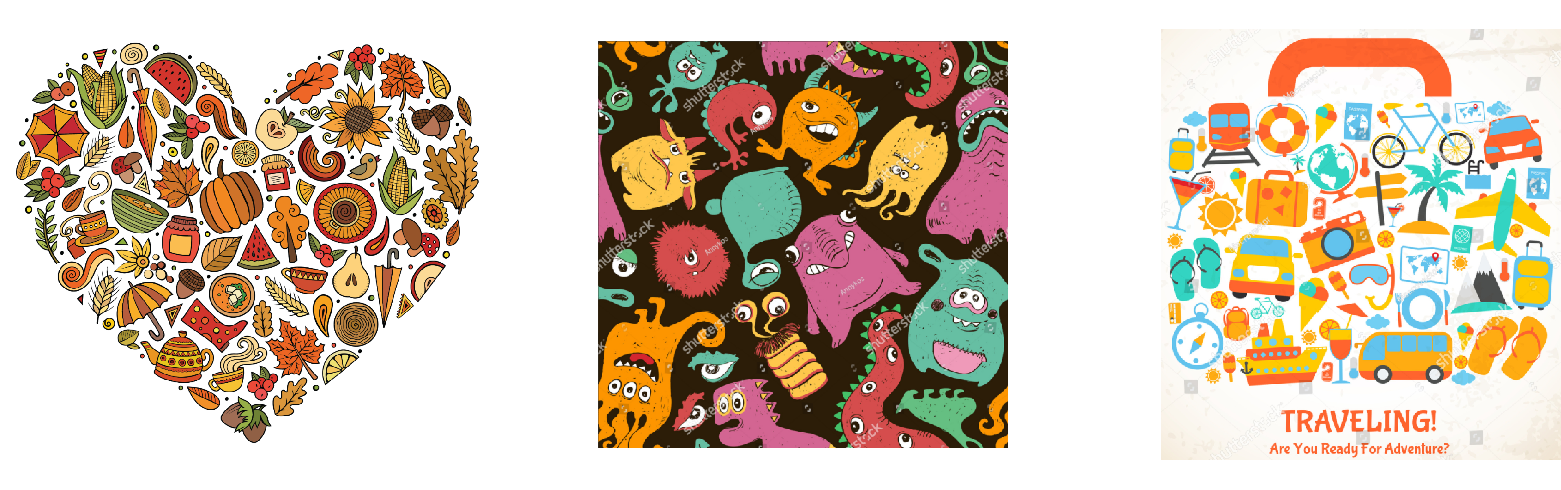
\includegraphics[width=1.0\textwidth]{figures/intro/graphics_designs.pdf} 
\caption{\label{fig_graphics_designs} 
Graphics designs. }
\end{figure}



\begin{figure}
\centering
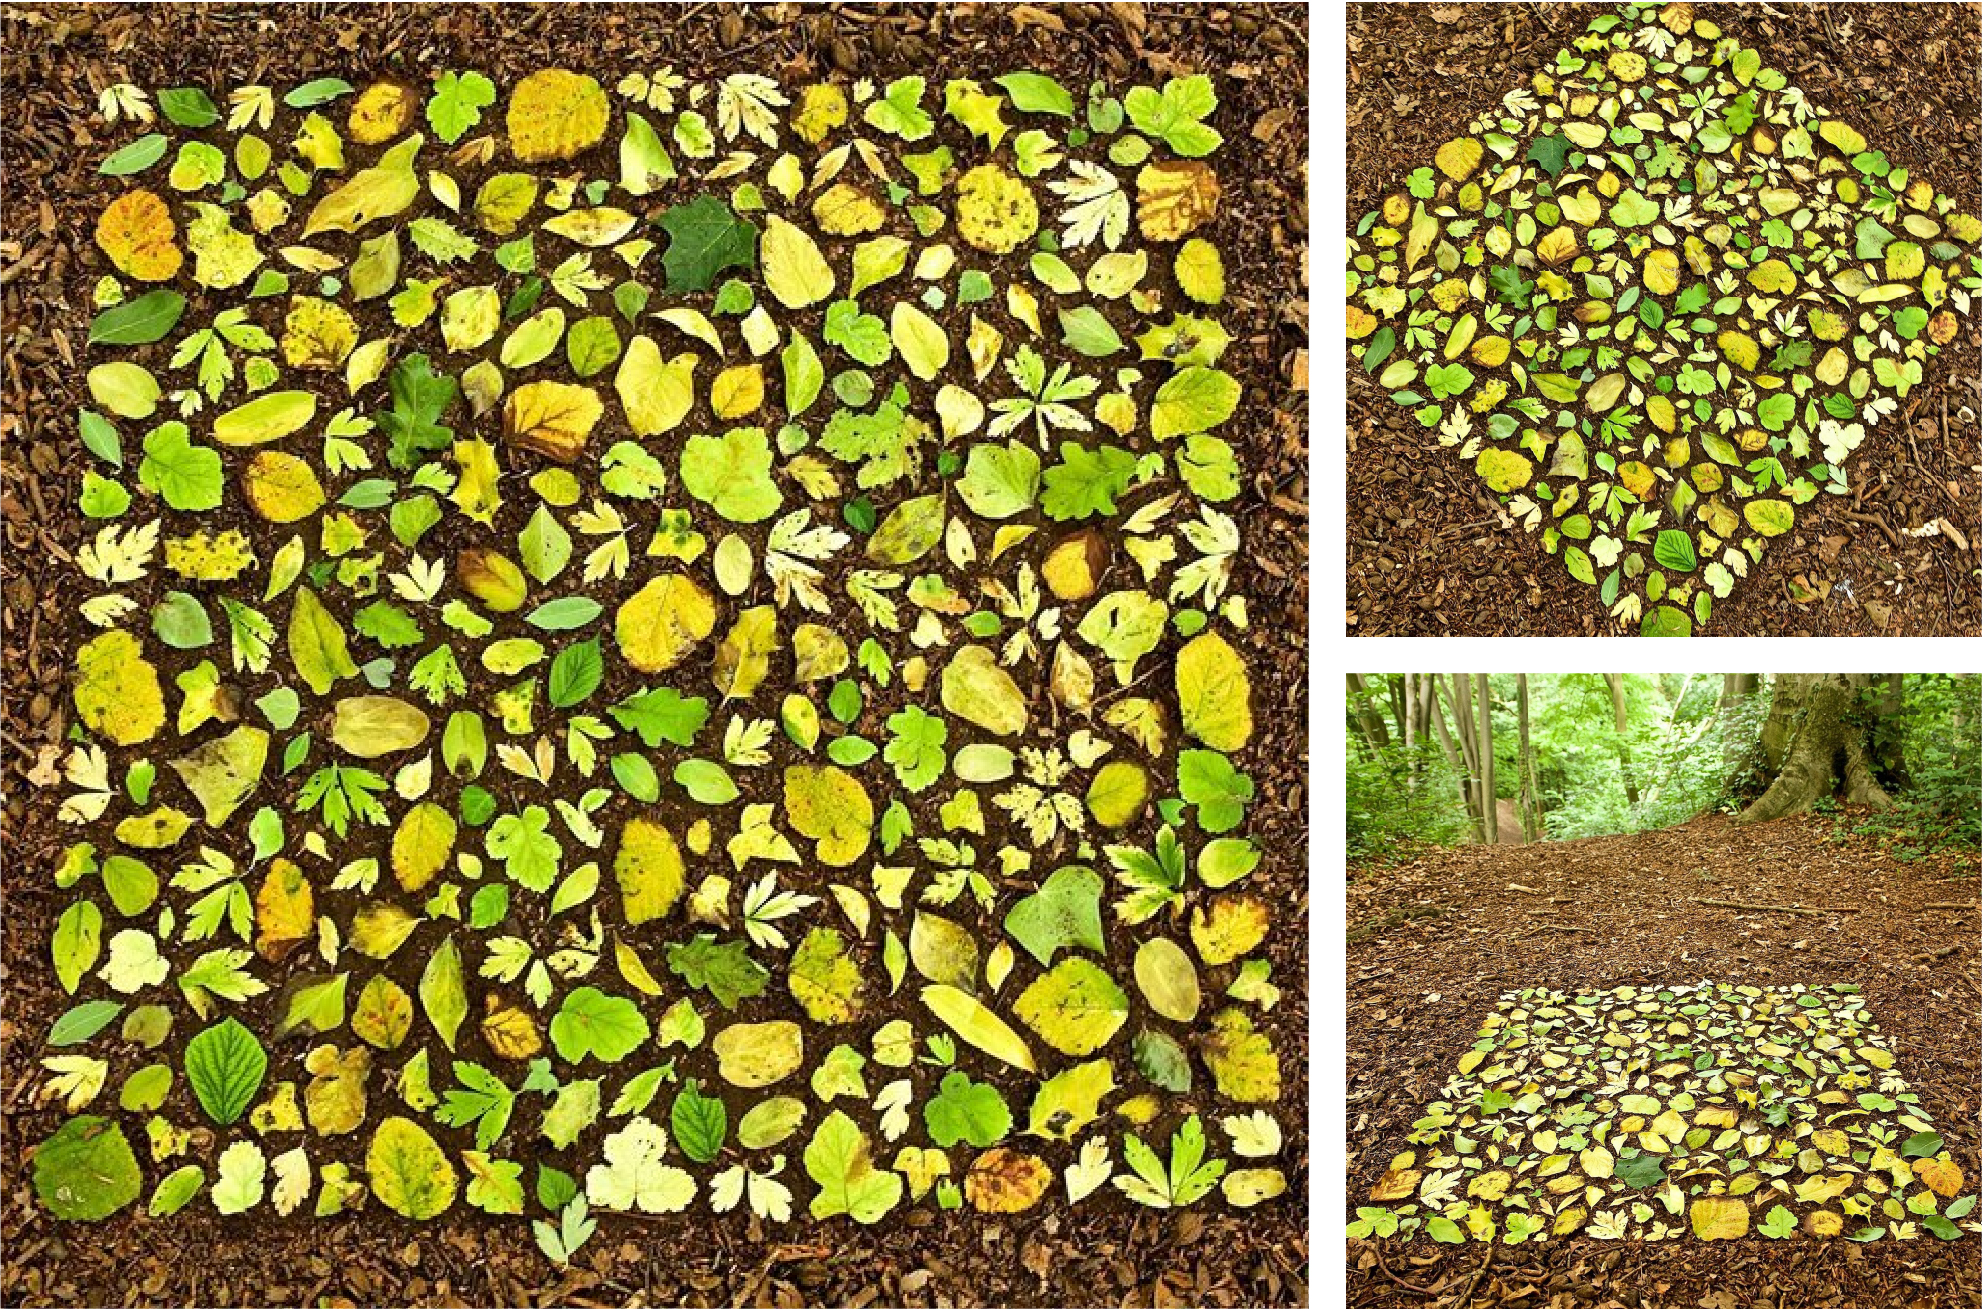
\includegraphics[width=0.5\textwidth]{figures/intro/woodland.jpg} 
\caption{\label{fig_woodland} 
Woodland. }
\end{figure}

\begin{figure}
\centering
\includegraphics[width=0.5\textwidth]{figures/intro/valve_lobby.jpg} 
\caption{\label{fig_valve_lobby} 
A packing installation in a lobby of a video game company. }
\end{figure}

\begin{figure}
\centering
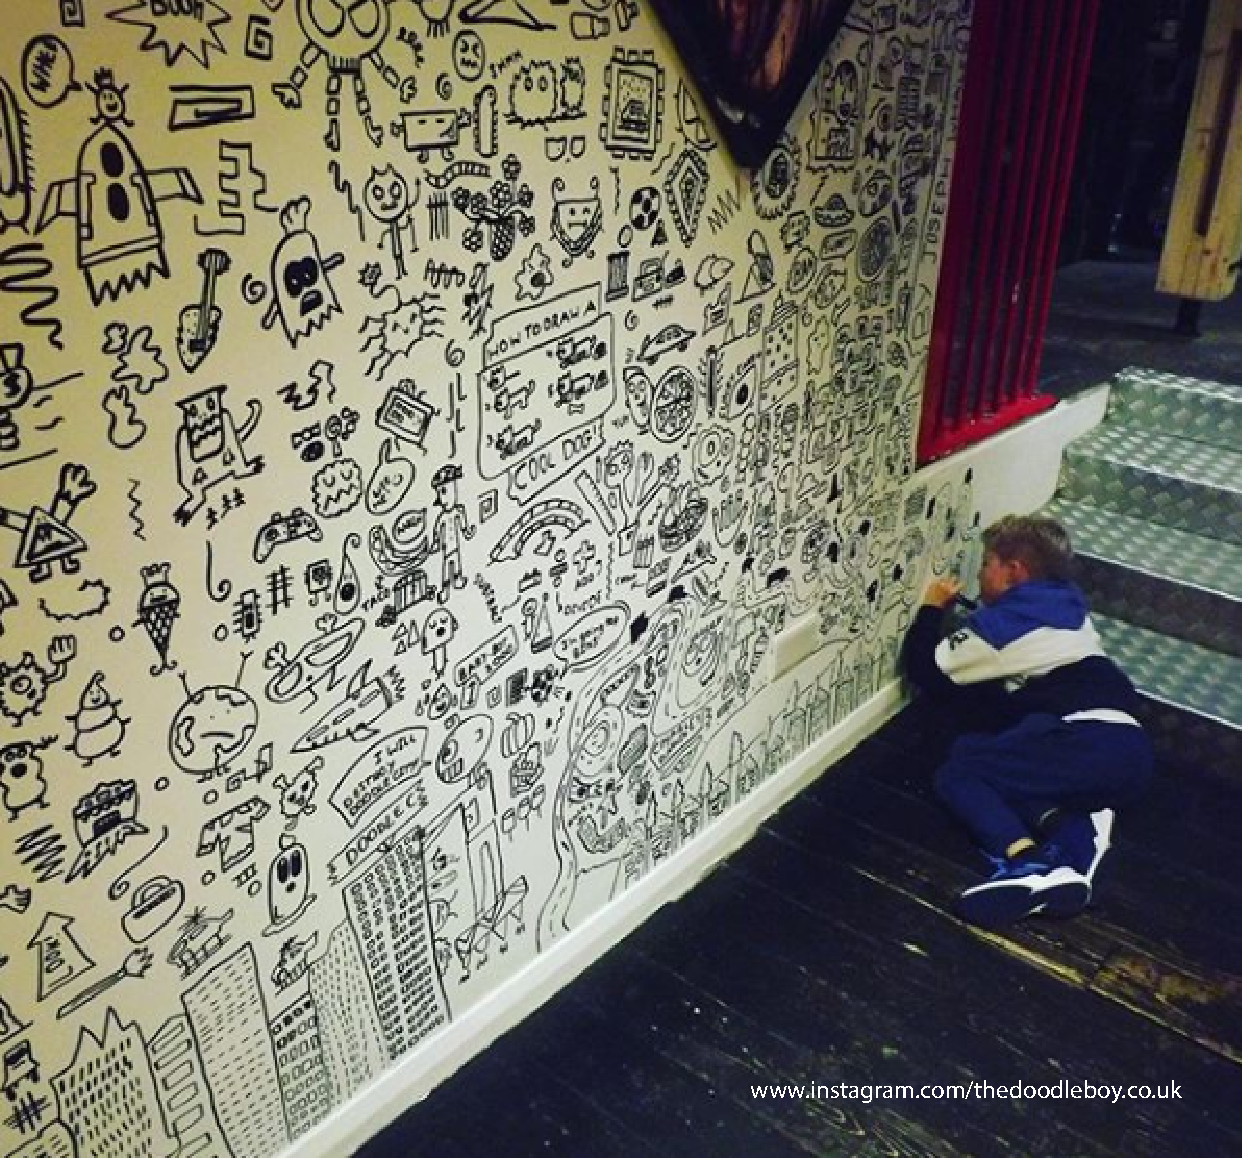
\includegraphics[width=0.5\textwidth]{figures/intro/doodle_boy.pdf} 
\caption{\label{fig_doodle_boy} 
Doodle boy. }
\end{figure}

\mynote{
Thesis Statement (one or two sentences)
\begin{itemize}
\item What is your thesis about and what have you done?
\item If you have a hypothesis what is it?
\item How will you test (prove/disprove) your hypothesis?
\end{itemize}
}


\mynote{Need to include illustrations of negative space}

\mynote{TODO: Copy from comp\_2}
A \textit{packing} is an arrangement of 2D geometric
\textit{elements} within a \textit{container} region in the plane.
Packings are popular in art, ornamentation, and graphics design.
Figure ~\ref{fig_logo_packings}\ref{fig_graphics_designs}\ref{fig_woodland}\ref{fig_valve_lobby}\ref{fig_doodle_boy} show several packing examples.
They can effectively convey a relationship between a unified whole (the
container shape) and its many sub-parts (the elements).

\mynote{maybe put negative space to the background section}
Elements are shapes like animals,
plants, geometric forms, or man-made objects.
An artist distributes elements so that they communicate
the shape of the container. 
The subset of the container that does not belong to any element is
called \textit{negative space}
(Fig.~\ref{packing_example}, right).
We can also interpret negative space as separation and gaps between elements.
The evenness of negative space plays an important role in 
packings.  
The artist should arrange elements in a way that their boundaries interlock with each other,
causing the separation between neighbouring elements to become roughly the same everywhere.
As the elements in a packing become perfectly interlocked,
the packing turns into a \textit{tiling}: a set of elements that exactly
fill a container with no overlaps and no negative space (Fig.~\ref{related_work_images}b).

\mynote{Motivation, Why is this problem you've worked on important}

\mynote{Goals / Objectives, What are you trying to do and why? 
How will you or the reader know if or when you've met your objectives?}

There has been a moderate amount of past research in computer
graphics, particularly in the field of non-photorealistic rendering,
on the generation of packings, tilings, or mosaics.  
See Chapter~\ref{related_work_section} for specific examples.  
However,  most techniques pack elements via rigid transformations, leading to
uneven element distribution and overlaps.  
Jigsaw Image Mosaics~\cite{Kim2002} and collages based on the Pyramid of Arclength
Descriptor~\cite{Kwan2016}, might be described as \textit{data-driven}.
These techniques rely on assembling a large library of elements, so that given an
area to fill in a partial composition, there is likely to be an
element in the library with a compatible shape.  The challenge is 
\textit{finding compatible elements}, 
which requires designing a shape descriptor that is fast and robust.
These techniques suppress imperfections by deforming
elements in a final post-processing step after they freeze the element positions.
The data-driven approaches do not always work.
They cannot guarantee to find a compatible element
at every iteration, and
elements typically do not fit perfectly with each other 
or the container boundary.
The remedy here is providing more data with increased computation time.
However, a large library may not be feasible or artistically desirable.
If an artist wants a packing of cats, and a data-driven approach 
cannot find a good result with ten cat shapes, 
the artist may not want to draw 100 or 1000 cat shapes to ensure a better fit.

\mynote{
Contributions, What is new, different, better, significant? Why is the world a better place because of what you've done? What have you contributed to the field of research?  What is now known/possible/better because of your thesis?
}

We propose \textit{deformation-driven} methods.
Instead of finding compatible elements,
we intend to \textit{create compatible elements} through element deformation
that can adapt to the shapes of neighboring elements and the container boundary.
We allow elements to deform in a controlled way,
to trade off between the evenness of the element distribution and 
the deformations of the individual elements.
By building an algorithm with a controllable deformation model at its core, we achieve a
more even distribution of negative space, even with a small library of element shapes.

Deformation-driven methods also allow us to work toward a design principle called \textit{uniformity amidst variety}~\cite{Hutcheson1729, Gombrich}. 
\textit{Uniformity} aims for an overall unity of design; 
\textit{variety} seeks to break up the monotony of
pure repetition.
We can achieve a degree of uniformity by using repeated copies of a small library of elements, but balance that uniformity with
variety by deforming those elements. 
We believe that there is a value in deformation that can generate plausible families of related elements from a single input shape.

\mynote {Explain briefly FLOWPAK, RepulsionPak, and AnimationPak.}